
\centerline{\textbf{ \LARGE Instruction Format}}

\begin{questyle}
  \question  For computers based on three-address instruction formats, each address field can be used
             to specify which of the following:  (GATE-2015\_Set\_1) \\
             S1: A memory operand \quad S2: A processor register \quad S3: An implied accumulator register

  \begin{oneparchoices}
    \CorrectChoice  Either S1 or S2
    \choice         Either S2 or S3
    \choice         Only S2 and S3
    \choice         S1, S2 and S3
  \end{oneparchoices}
\end{questyle}


\begin{questyle}
  \question  A processor has 40 distinct instructions and 24 general purpose registers.
             A 32-bit instruction word has an opcode, two register operands and an immediate operand.
             The number of bits available for the immediate operand field is \fillin[16] (GATE-2016\_Set\_2)
             \\ Hint : \qquad 5-bits to index 24 register \qquad 6-bis to index 40 opcode
             \\ HInt : \qquad Instruction(32 bit) = opcode(6) + R1(5) + R2(5) + Immediate Operand(x)
\end{questyle}

\begin{questyle}
  \question  A machine has a 32-bit architecture, with 1-word long instructions. It has 64 registers,
             each of which is 32 bits long. It needs to support 45 instructions, which have an immediate
             operand in addition to two register operands. Assuming that the immediate operand is an
             unsigned integer, the maximum value of the immediate operand is
             \fillin[16383 \( \boldsymbol {(2^{14} -1)} \)] (GATE-2014\_Set\_1)
             \\ Hint : \qquad 6-bits to index 64 register \qquad 6-bis to index 45 opcode(instructions)
             \\ HInt : \qquad Instruction(32 bit) = opcode(6) + R1(6) + R2(6) + Immediate Operand(x)
\end{questyle}

\begin{questyle}
  \question  Consider a processor with 64 registers and an instruction set of size twelve. Each
             instruction has five distinct fields, namely, opcode, two source register identifiers,
             one destination register identifier, and a twelve-bit immediate value. Each instruction
             must be stored in memory in a byte-aligned fashion. If a program has 100 instructions,
             the amount of memory (in bytes) consumed by the program text is \fillin[500] (GATE-2016\_Set\_2)
             \\ Hint : \quad 6-bits to index 64 register \qquad 4-bis to index 12 opcode(instructions)
             \\ Hint : \quad Instruction(34 bit) = opcode(4) + R1(6) + R2(6) + R3(6) + Immediate Operand(12)
             \\ Hint : \quad Total size need to store one instruction in byte-aligned fashion = 40(\(\thickapprox\)34) = 5 bytes.
             \\ Hint : \quad Size to store 100 instructions = 5 x 100 = 500 Bytes
\end{questyle}


\begin{questyle}
  \question  The microinstructions stored in the control memory of a processor have a width of 26 bits.
             Each microinstruction is divided into three fields: a micro-operation field of 13 bits, a
             next address field (X), and a MUX select field (Y). There are 8 status bits in the inputs
             of the MUX.  How many bits are there in the X and Y fields, and what is the size of the
             control memory in number of words? (GATE-2004)(SP – 1)

             \begin{myTableStyle} \begin{tabular}{ |m{14cm}| } \hline
                  \begin{center} 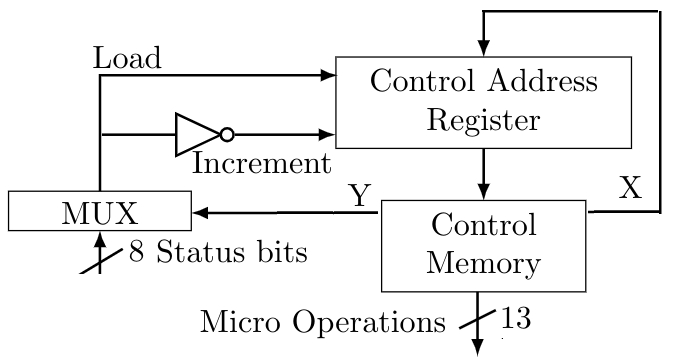
\includegraphics[scale=0.4]{./images/control_memory.jpeg} \end{center}\\ \hline
            \end{tabular} \end{myTableStyle} \vspace{0.08in}

  \begin{oneparchoices}
    \CorrectChoice  10, 3, 1024
    \choice         8, 5, 256
    \choice         5, 8, 2048
    \choice         10, 3, 512
  \end{oneparchoices}
  \\Hint: \quad X + Y + 13 = 26
  \\Hint: \quad Y = 3  \qquad 3 select bits are needed to select 8 i/p lines of MUX
  \\Hint: \quad X = 10 \qquad Size of Control memory = \( \mathbf { 2^{10} } \) Words
\end{questyle}


\begin{comment}

\begin{questyle}
  \question  zzz  (GATE-zzz)

  \begin{choices}
    \choice         zzz
    \choice         zzz
    \choice         zzz
    \choice         zzz
\CorrectChoice
  \end{choices}
\end{questyle}

\begin{questyle}
  \question  zzz  (GATE-zzz)

  \begin{choices}
    \choice         zzz
    \choice         zzz
    \choice         zzz
    \choice         zzz
\CorrectChoice
  \end{choices}
\end{questyle}

\begin{questyle}
  \question  zzz  (GATE-zzz)

  \begin{choices}
    \choice         zzz
    \choice         zzz
    \choice         zzz
    \choice         zzz
\CorrectChoice
  \end{choices}
\end{questyle}

\end{comment}






